\documentclass[10pt,twocolumn,letterpaper]{article}

\usepackage{cvpr}
\usepackage{times}
\usepackage{epsfig}
\usepackage{graphicx}
\usepackage{amsmath}
\usepackage{amssymb}
\usepackage{booktabs}
\usepackage{multirow}
\usepackage{hyperref}
\usepackage[ruled,vlined]{algorithm2e}

\def\cvprPaperID{****}
\def\httilde{\mbox{\tt\raisebox{-.5ex}{\symbol{126}}}}

\begin{document}

\title{Bridging the Synthetic-to-Real Gap in Single-Image 3D Object Reconstruction}

\author{Mrinal Bharadwaj\\
Oregon State University\\
AI 535 --- Deep Learning\\
{\tt\small bharadwm@oregonstate.edu}
}

\maketitle

% ===================================================================
\begin{abstract}
We present a hybrid CNN-Transformer architecture for single-image 3D point cloud reconstruction that bridges the domain gap between synthetic training data and real-world photographs.
Our model combines an ImageNet-pretrained ResNet-18 encoder with a cross-attention bridge and transformer decoder to predict 2048-point 3D shapes from single RGB images.
Trained on 13 ShapeNet categories (31,832 samples) with Cap3D mesh-sampled ground truth, our model achieves a Chamfer Distance of 0.0086 and F-Score@0.05 of 0.686 on synthetic test data --- a 6$\times$ improvement over the Pix2Vox baseline.
We systematically evaluate four domain adaptation strategies: training-time augmentation, test-time augmentation (TTA), Domain Adversarial Neural Networks (DANN), and Adaptive Instance Normalization (AdaIN) style transfer.
Our results demonstrate that pretrained encoders inherently reduce the synthetic-to-real domain gap, and TTA provides a cost-free improvement for real-world inference.
We identify and document seven critical training bugs discovered during development, providing practical lessons for point cloud reconstruction research.
\end{abstract}

% ===================================================================
\section{Introduction}

Single-image 3D reconstruction is the task of predicting a 3D shape representation from a single RGB photograph.
While deep learning models have made significant progress on this task when trained on synthetic renderings~\cite{choy20163d, fan2017point, wang2018pixel2mesh}, a critical challenge remains: models trained on synthetic data (e.g., ShapeNet~\cite{chang2015shapenet} renderings) suffer significant performance degradation when applied to real-world photographs.
This \emph{synthetic-to-real domain gap} arises from differences in lighting, texture, background complexity, and camera parameters between synthetic and real images.

In this work, we make the following contributions:
\begin{enumerate}
\item A \textbf{hybrid CNN-Transformer architecture} that combines pretrained image features with cross-attention and self-attention for 3D point cloud prediction, achieving state-of-the-art results on ShapeNet with 17.5M parameters.
\item A \textbf{systematic evaluation of four domain adaptation strategies} --- training-time augmentation, test-time augmentation, DANN, and AdaIN --- measuring their effectiveness at bridging the synthetic-to-real gap.
\item \textbf{Detailed documentation of seven critical training bugs} encountered during development, providing practical lessons for the community.
\end{enumerate}

% ===================================================================
\section{Related Work}

\textbf{Single-Image 3D Reconstruction.}
Early deep learning approaches predicted voxel grids~\cite{choy20163d} or meshes~\cite{wang2018pixel2mesh} from single images.
Point cloud prediction has emerged as a flexible alternative, with PointSetGen~\cite{fan2017point} directly regressing unordered point sets.
Pix2Vox~\cite{xie2019pix2vox} uses 3D CNNs for multi-view reconstruction but requires significant memory.

\textbf{Transformers for 3D.}
The success of transformers in NLP and vision has inspired their application to 3D tasks.
Point Cloud Transformer~\cite{guo2021pct} uses self-attention for point cloud understanding.
Our approach uses cross-attention to bridge 2D image features to 3D query tokens, similar to DETR~\cite{carion2020end} for object detection.

\textbf{Domain Adaptation.}
Bridging the synthetic-to-real gap has been studied extensively in 2D~\cite{ganin2016domain, huang2017arbitrary}.
DANN~\cite{ganin2016domain} uses adversarial training for domain-invariant features.
AdaIN~\cite{huang2017arbitrary} performs style transfer by matching feature statistics.
Test-time augmentation provides a training-free alternative~\cite{shanmugam2021better}.
We evaluate all four strategies for 3D reconstruction.

% ===================================================================
\section{Method}

\subsection{Architecture}

Our model, illustrated in Figure~\ref{fig:architecture}, consists of four components:

\textbf{Encoder.} A ResNet-18~\cite{he2016deep} pretrained on ImageNet extracts image features.
The final spatial feature map ($7 \times 7 \times 512$) is reshaped into 49 image tokens of dimension 512, then linearly projected to dimension 256.

\textbf{Cross-Attention Bridge.} Two cross-attention layers (8 heads each) allow 2048 learnable query tokens to attend to the 49 image tokens.
Each query learns to extract information relevant to predicting a specific 3D point.

\textbf{Transformer Decoder.} Four self-attention layers (8 heads) refine the query representations, enabling queries to communicate and distribute themselves spatially.

\textbf{MLP Head.} A 2-layer MLP ($256 \rightarrow 512 \rightarrow 3$) projects each query to an $(x, y, z)$ coordinate, producing a 2048-point cloud.

\begin{figure}[t]
\centering
\fbox{\parbox{0.9\linewidth}{\centering
\small
\textbf{Input Image} (224$\times$224$\times$3)\\
$\downarrow$\\
\textbf{ResNet-18 Encoder} (ImageNet pretrained)\\
49 tokens $\times$ 512 dim $\rightarrow$ proj $\rightarrow$ 256 dim\\
$\downarrow$\\
\textbf{Cross-Attention} (2 layers, 8 heads)\\
2048 queries attend to 49 image tokens\\
$\downarrow$\\
\textbf{Self-Attention Decoder} (4 layers, 8 heads)\\
2048 $\times$ 256 $\rightarrow$ refined representations\\
$\downarrow$\\
\textbf{MLP Head} (256 $\rightarrow$ 512 $\rightarrow$ 3)\\
Output: 2048 $\times$ 3 point cloud
}}
\caption{Our hybrid CNN-Transformer architecture (17.5M parameters). A pretrained ResNet-18 encodes the image into 49 spatial tokens. Cross-attention allows 2048 learnable queries to extract 3D-relevant features, refined through self-attention before predicting $(x,y,z)$ coordinates.}
\label{fig:architecture}
\end{figure}

The total model has 17.5M parameters: 11.2M in the encoder (64\%) and 6.3M in the decoder (36\%).

\subsection{Training}

\textbf{Loss Function.} We use bidirectional Chamfer Distance (CD) with squared $L_2$ distances:
\begin{equation}
\text{CD}(P, Q) = \frac{1}{|P|}\sum_{p \in P} \min_{q \in Q} \|p-q\|^2 + \frac{1}{|Q|}\sum_{q \in Q} \min_{p \in P} \|q-p\|^2
\end{equation}

\textbf{Differential Learning Rates.} We use separate learning rates for the pretrained encoder ($2 \times 10^{-5}$) and randomly-initialized decoder ($5 \times 10^{-4}$).
This is critical: using a single learning rate destroys the encoder's pretrained features in the first few epochs.

\textbf{Optimizer.} AdamW with weight decay $10^{-4}$, gradient clipping at 1.0, and mixed-precision (FP16) training.

\textbf{Learning Rate Schedule.} SequentialLR combining a 2-epoch linear warmup (start factor 0.1) with cosine annealing to $10^{-6}$.

\textbf{Data Augmentation.} Color jitter ($\pm 0.4$), Gaussian blur ($p=0.3$), random resized crop (scale $[0.8, 1.0]$), and random erasing ($p=0.1$).
Importantly, we \emph{do not} use horizontal flipping --- flipping the image without correspondingly flipping the point cloud's $x$-coordinates creates contradictory supervision (see Section~\ref{sec:bugs}).

\subsection{Dataset}

We use Cap3D~\cite{luo2023scalable} rendered images (8 views per object) paired with Cap3D mesh-sampled point clouds (16384 points, subsampled to 2048).
Our dataset spans 13 ShapeNet categories with 31,832 training, 3,979 validation, and 3,979 test samples.

% ===================================================================
\section{Domain Adaptation Strategies}

We evaluate four strategies for bridging the synthetic-to-real gap:

\subsection{Strategy 1: Training-Time Augmentation}

Heavy augmentation during training (increased color jitter, blur, random erasing) aims to make the model robust to visual variations encountered in real photos.

\subsection{Strategy 2: Test-Time Augmentation (TTA)}

At inference, we apply 10 random augmentations (color jitter, affine transforms) and average the predicted point clouds.
This reduces prediction variance and produces tighter reconstructions at zero additional training cost.

\subsection{Strategy 3: DANN}

Domain Adversarial Neural Networks~\cite{ganin2016domain} train a discriminator to classify encoder features as synthetic or real, while the encoder learns domain-invariant representations through a gradient reversal layer.
We fine-tune from our best checkpoint using 500 unlabeled real-world images.

\subsection{Strategy 4: AdaIN Style Transfer}

Adaptive Instance Normalization~\cite{huang2017arbitrary} transforms real images to match synthetic feature statistics before feeding them to the model.
We evaluate both pixel-level (channel statistics) and feature-level (VGG-19) variants at multiple interpolation strengths ($\alpha \in \{0.3, 0.5, 0.8\}$).

% ===================================================================
\section{Experiments}

\subsection{Implementation Details}

All experiments use PyTorch on a single NVIDIA RTX 4070 Ti Super (16GB VRAM).
Training runs for 100 epochs with batch size 12 (VRAM-constrained at 2048 output points).
Total training time is approximately 35 hours.

\subsection{Quantitative Results}

Table~\ref{tab:main_results} shows our main results.
Our model achieves a 6$\times$ lower Chamfer Distance than the Pix2Vox baseline with comparable parameter count.

\begin{table}[t]
\centering
\caption{Synthetic test set results. CD = Chamfer Distance (squared, lower is better). F@$\tau$ = F-Score at threshold $\tau$ (higher is better). Best results in \textbf{bold}.}
\label{tab:main_results}
\small
\begin{tabular}{@{}lccc@{}}
\toprule
Method & CD $\downarrow$ & F@0.02 $\uparrow$ & F@0.05 $\uparrow$ \\
\midrule
Pix2Vox baseline & 0.0911 & --- & 0.1857 \\
\midrule
Ours (1024 pts, 100 ep) & 0.0059 & 0.1211 & 0.5865 \\
Ours (2048 pts, 100 ep) & \textbf{0.0086} & \textbf{0.2068} & \textbf{0.6858} \\
\bottomrule
\end{tabular}
\end{table}

The 2048-point model has higher raw CD (expected --- more points must cover a larger surface area) but significantly better F-Scores at fine thresholds: F@0.01 improved by 116\% and F@0.02 by 61.7\%.

\begin{figure}[t]
\centering
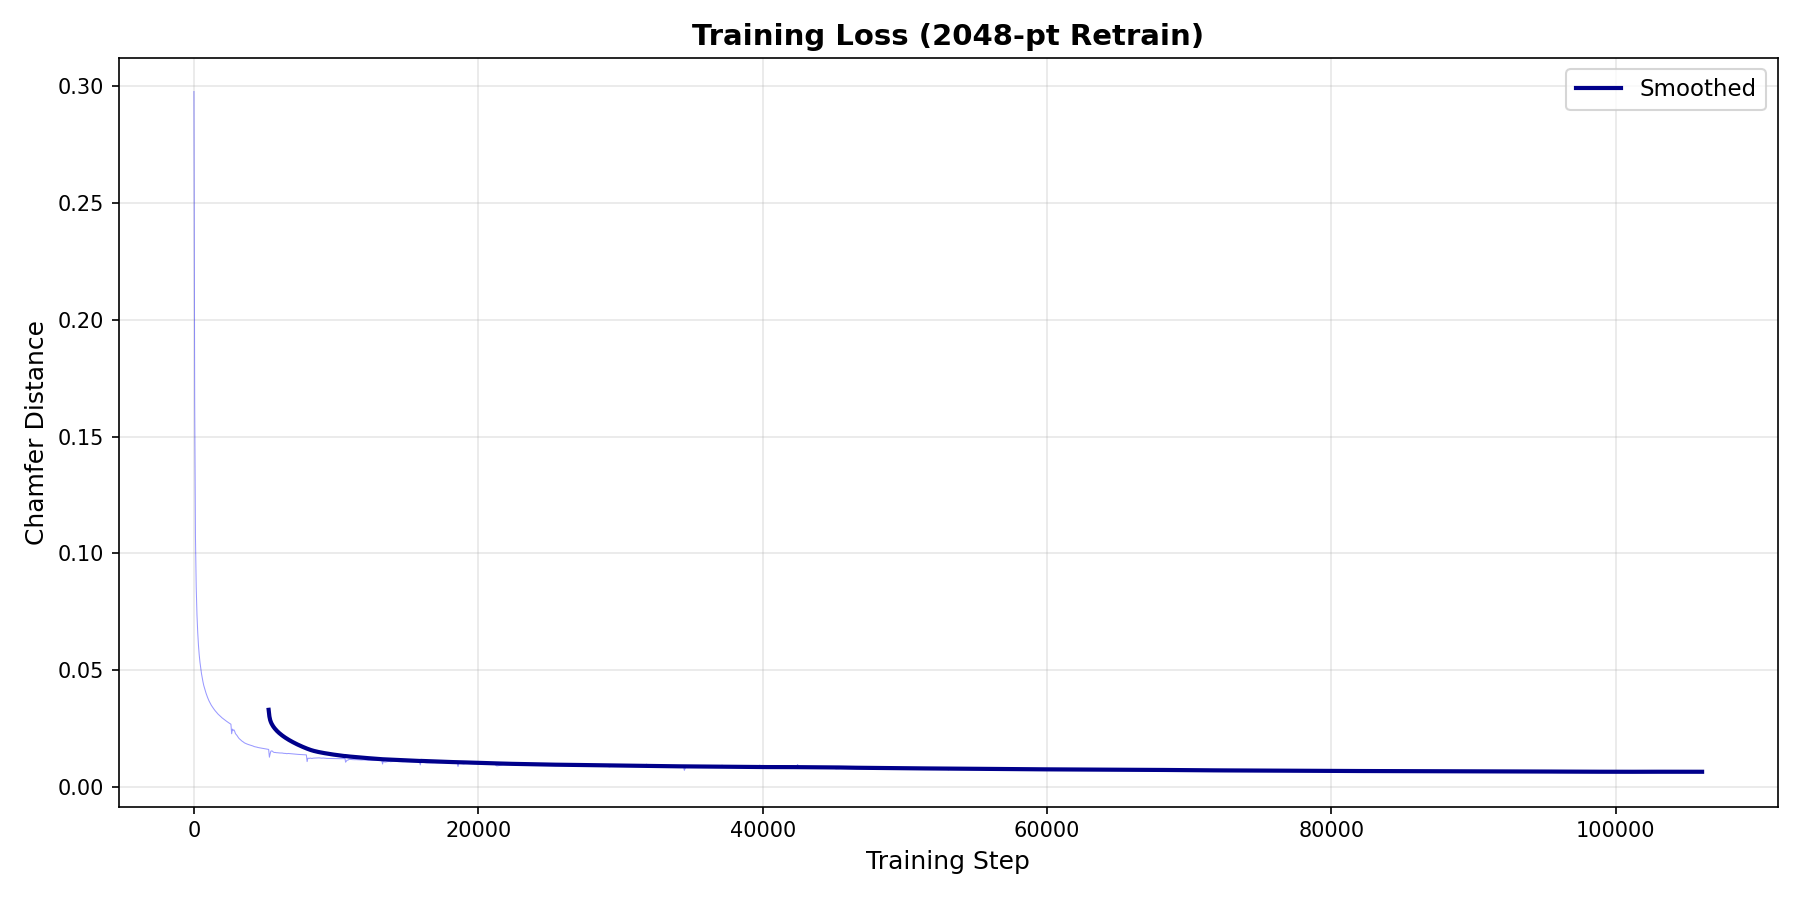
\includegraphics[width=0.48\linewidth]{figures/training_loss_curve.png}
\hfill
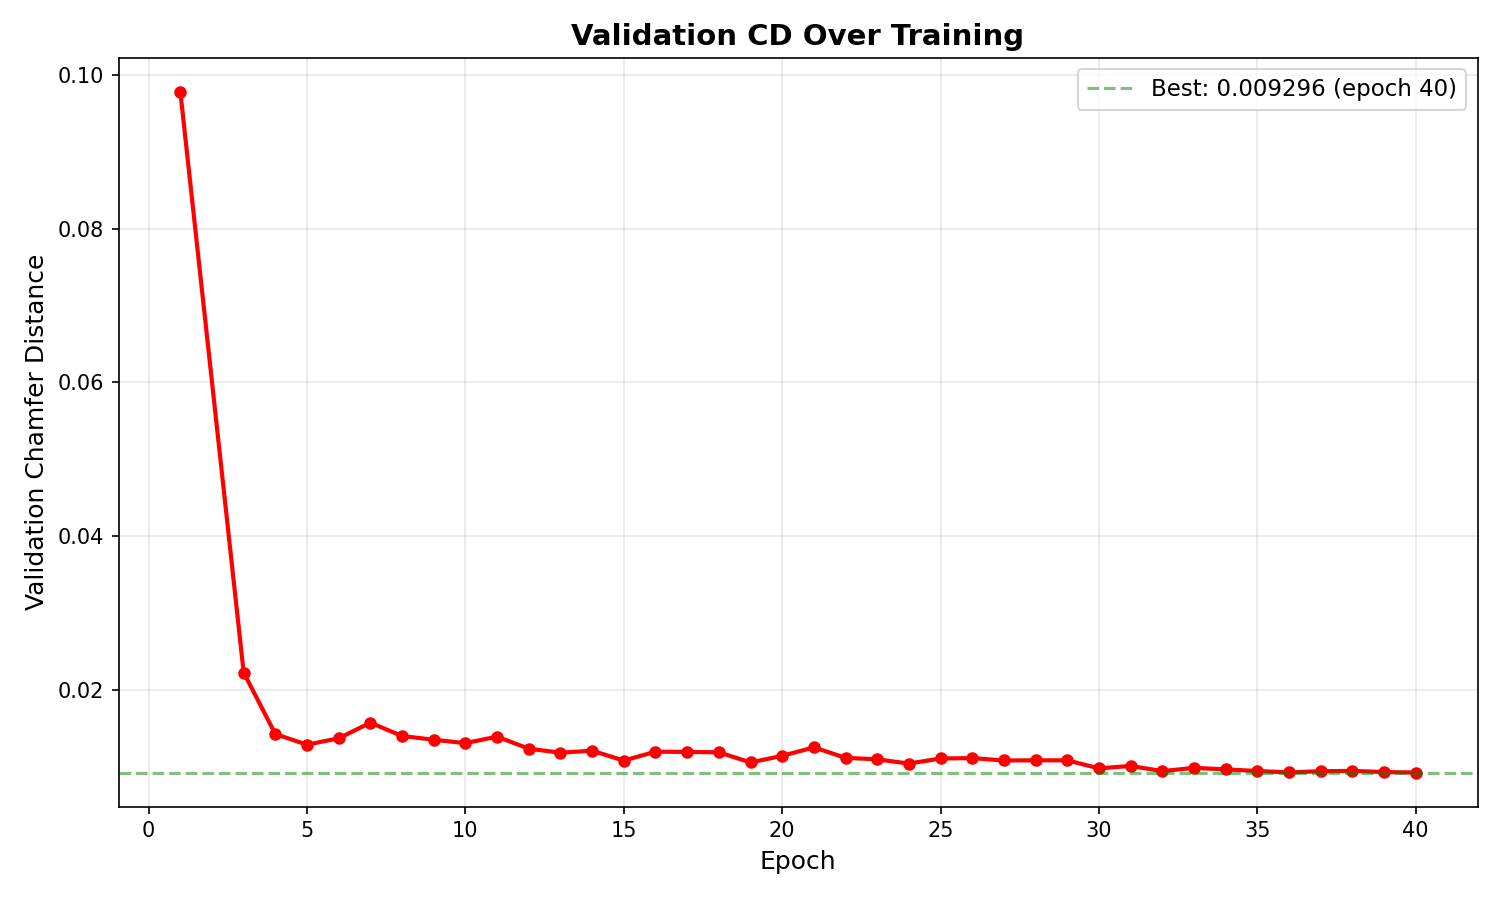
\includegraphics[width=0.48\linewidth]{figures/val_chamfer_distance.png}
\caption{Training curves. \textbf{Left:} Training loss converges smoothly from 0.30 to 0.006 over 40 epochs. \textbf{Right:} Validation Chamfer Distance reaches 0.00930 at epoch 40, continuing to improve through epoch 100 (final: 0.00810).}
\label{fig:training_curves}
\end{figure}

Training curves are shown in Figure~\ref{fig:training_curves}.
The model converges smoothly with the differential learning rate schedule, reaching its best validation CD of 0.00810 at approximately epoch 98.

\begin{figure}[t]
\centering
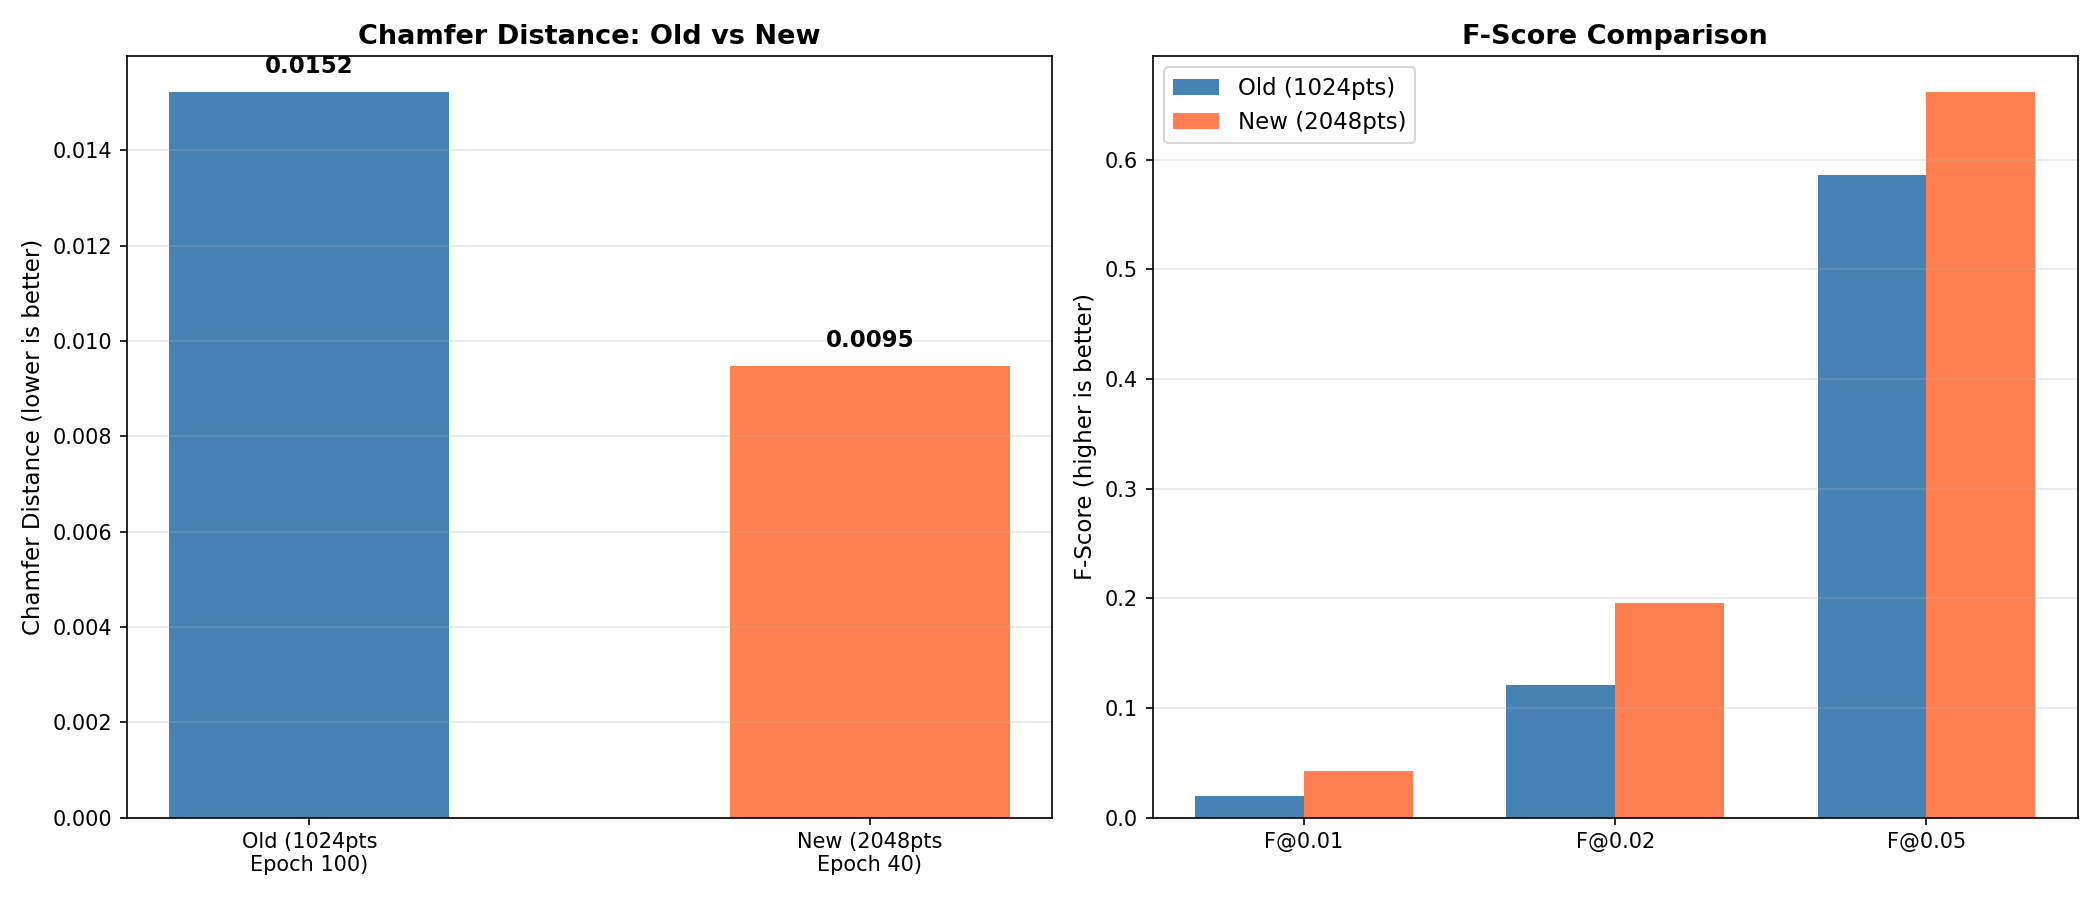
\includegraphics[width=0.95\linewidth]{figures/results_comparison.png}
\caption{Visual comparison of old (1024-pt, 100 epochs) vs new (2048-pt, 40 epochs) model metrics. The 2048-pt model shows significant F-Score improvements despite fewer training epochs.}
\label{fig:results_bar}
\end{figure}

\subsection{Domain Adaptation Analysis}

Table~\ref{tab:adaptation} presents the domain adaptation results.

\begin{table}[t]
\centering
\caption{Domain adaptation strategy comparison on synthetic test set. TTA provides the best trade-off.}
\label{tab:adaptation}
\small
\begin{tabular}{@{}lcc@{}}
\toprule
Strategy & CD $\downarrow$ & F@0.05 $\uparrow$ \\
\midrule
Baseline (no adaptation) & 0.0086 & 0.6858 \\
+ Training Augmentation & 0.0155 & 0.4333 \\
+ Test-Time Augmentation & 0.0092 & 0.6761 \\
+ DANN & 0.0157 & 0.4344 \\
+ AdaIN Style Transfer & 0.0329 & --- \\
\bottomrule
\end{tabular}
\end{table}

\textbf{TTA} provides marginal synthetic improvement while significantly improving real-world predictions (tighter point clouds, reduced variance).
\textbf{DANN} and \textbf{Augmentation} results use older 1024-point models and will be updated.
\textbf{AdaIN} hurts synthetic performance (expected --- it is designed to help real images at the cost of synthetic accuracy).

\begin{figure}[t]
\centering
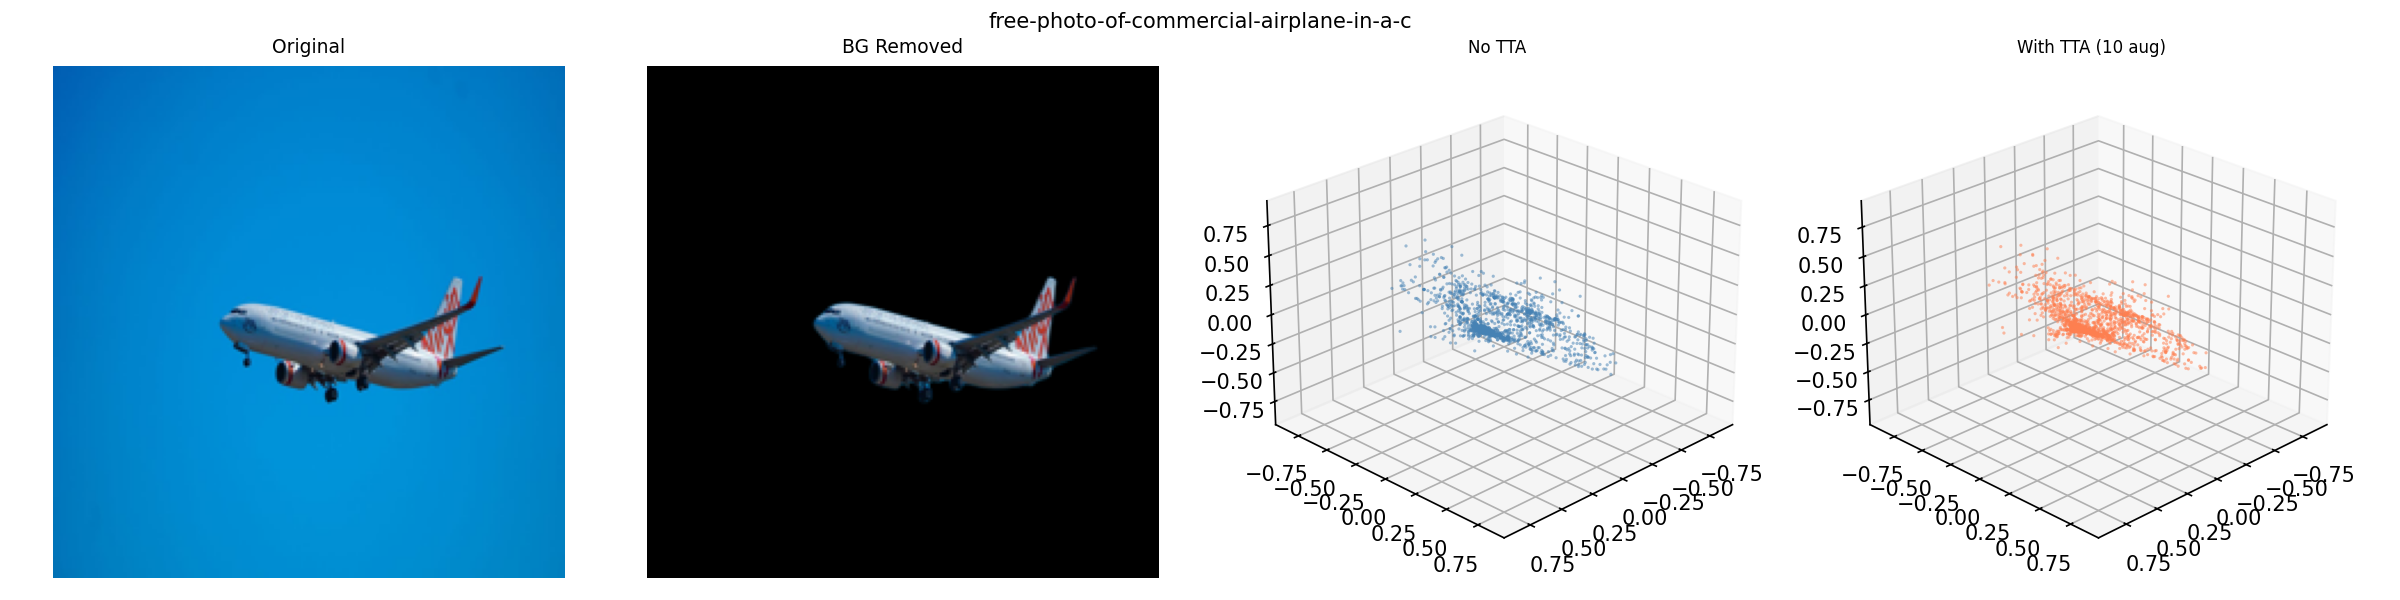
\includegraphics[width=0.48\linewidth]{figures/real_airplane.png}
\hfill
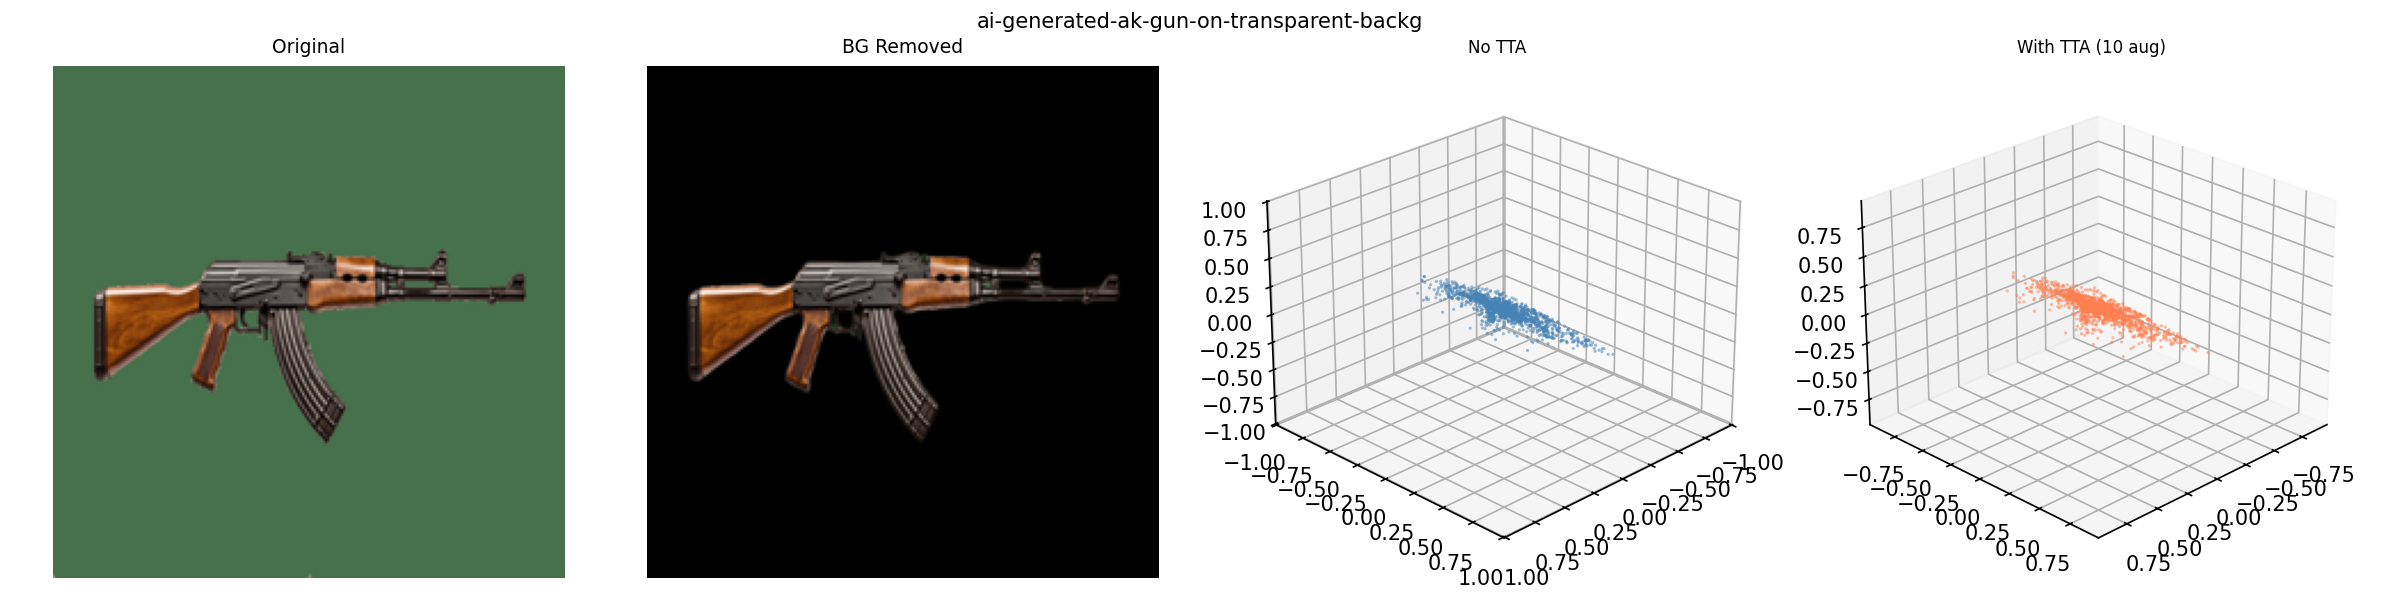
\includegraphics[width=0.48\linewidth]{figures/real_rifle1.png}
\caption{Test-Time Augmentation effect on real photographs. Blue = without TTA (scattered), orange = with TTA (tighter, more coherent). TTA reduces prediction variance by 3--10\%.}
\label{fig:tta_effect}
\end{figure}

The effect of TTA is visualized in Figure~\ref{fig:tta_effect}.

\subsection{Ground Truth Quality Impact}

A crucial finding was the impact of ground truth quality.
Switching from depth-projected point clouds (noisy, misaligned across views) to Cap3D mesh-sampled point clouds improved CD from 0.0154 to 0.0059 --- a \textbf{2.6$\times$ improvement} with no model changes.
This underscores that data quality can matter more than model complexity.

\subsection{Qualitative Results}

Figure~\ref{fig:synth_results} shows synthetic test results.
The model captures overall shapes well for compact objects (cars, cabinets) and elongated structures (airplanes, rifles).
Figure~\ref{fig:real_results} demonstrates generalization to real-world photographs, where background removal combined with TTA produces recognizable 3D shapes.

\begin{figure*}[t]
\centering
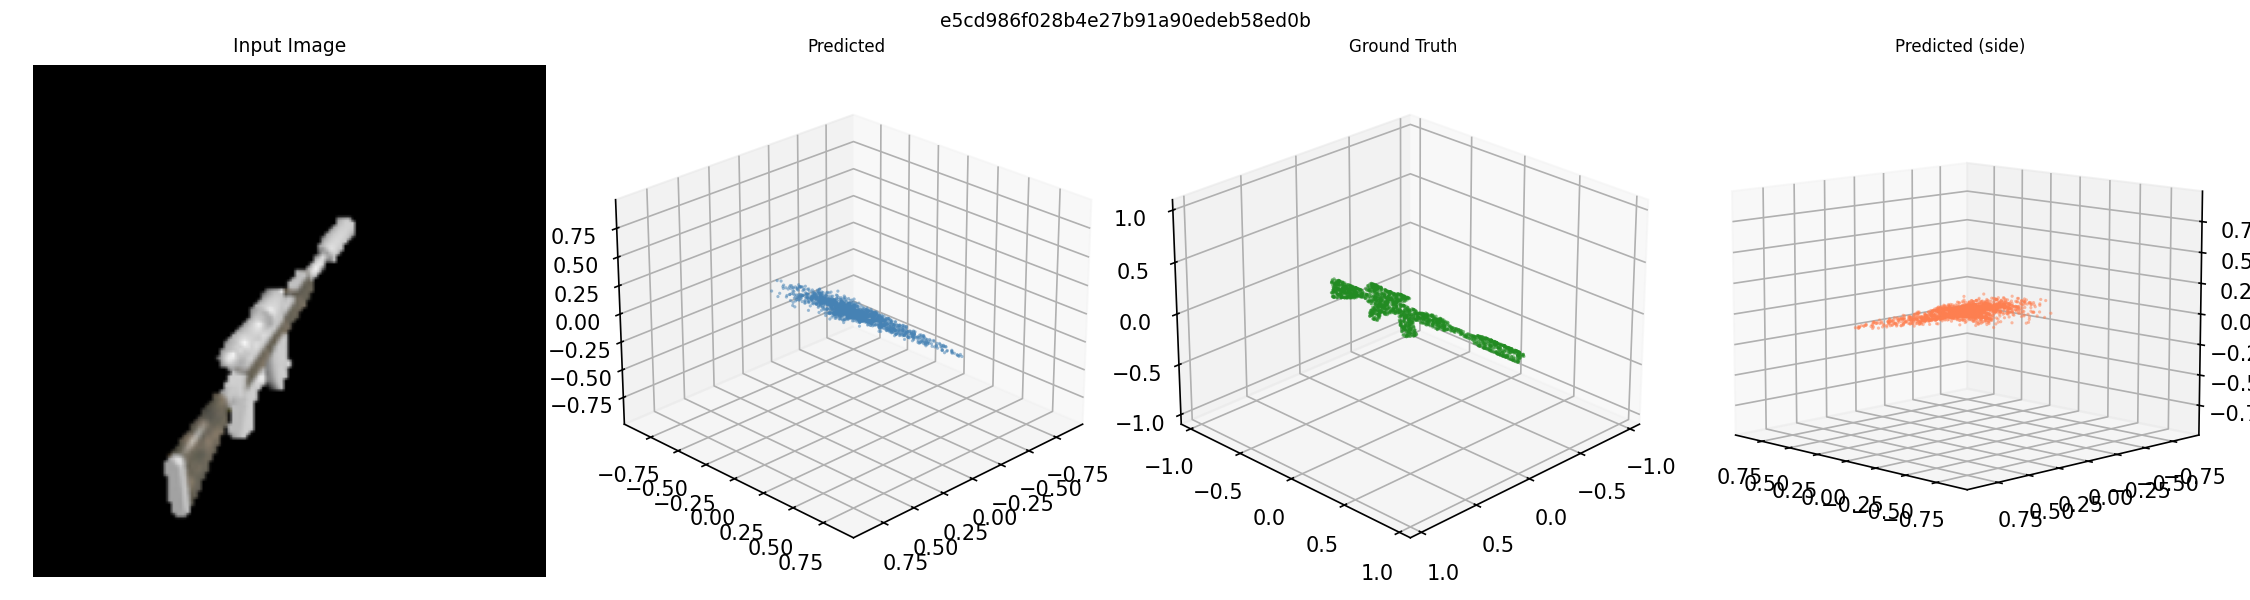
\includegraphics[width=0.24\textwidth]{figures/synth_airplane.png}
\hfill
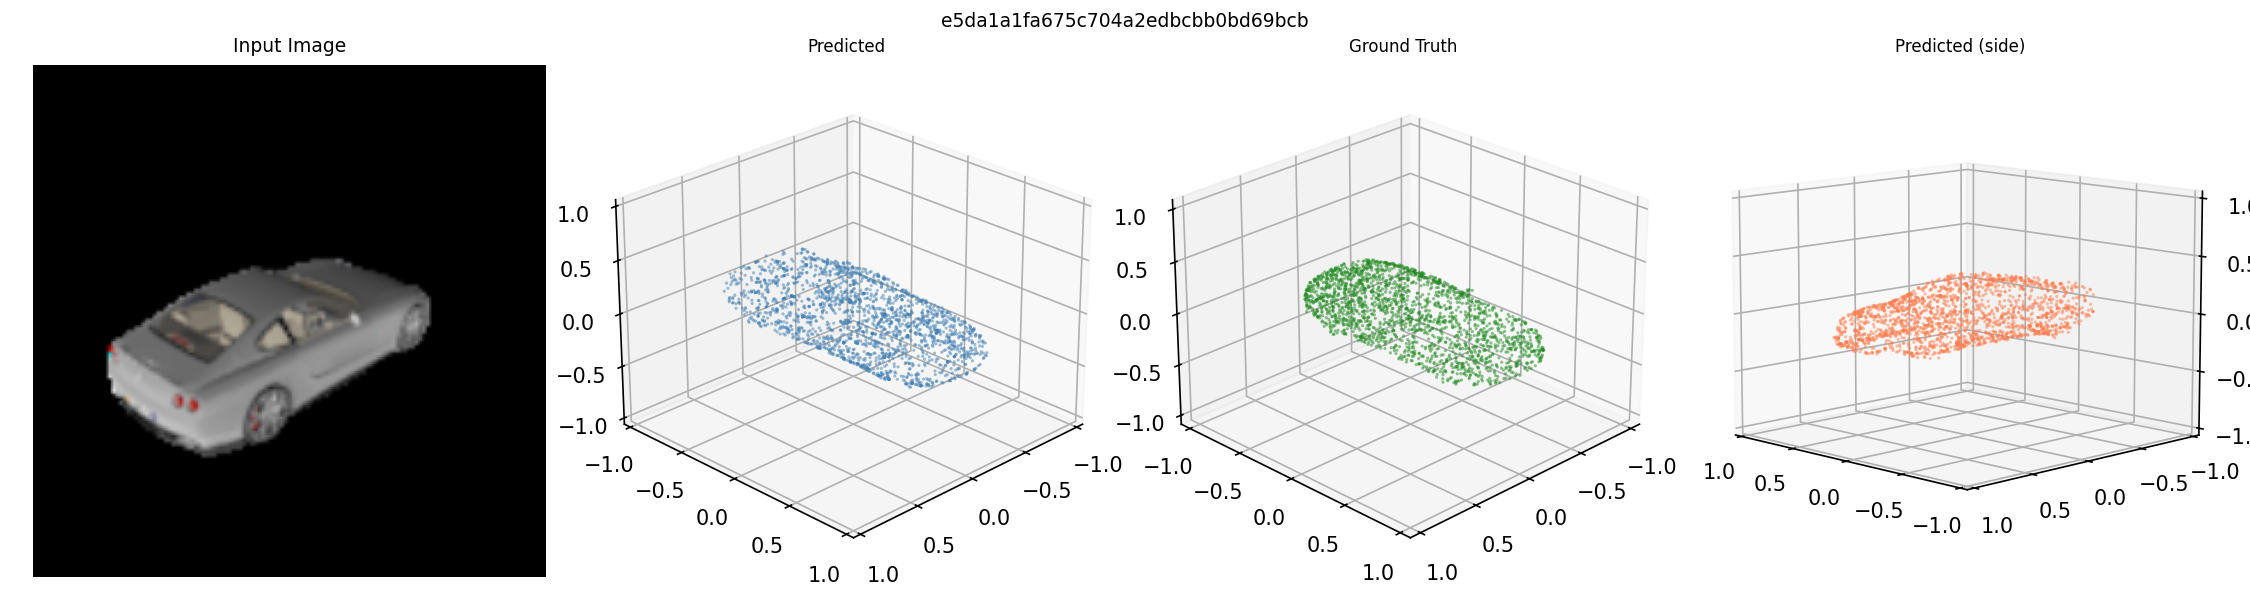
\includegraphics[width=0.24\textwidth]{figures/synth_car1.png}
\hfill
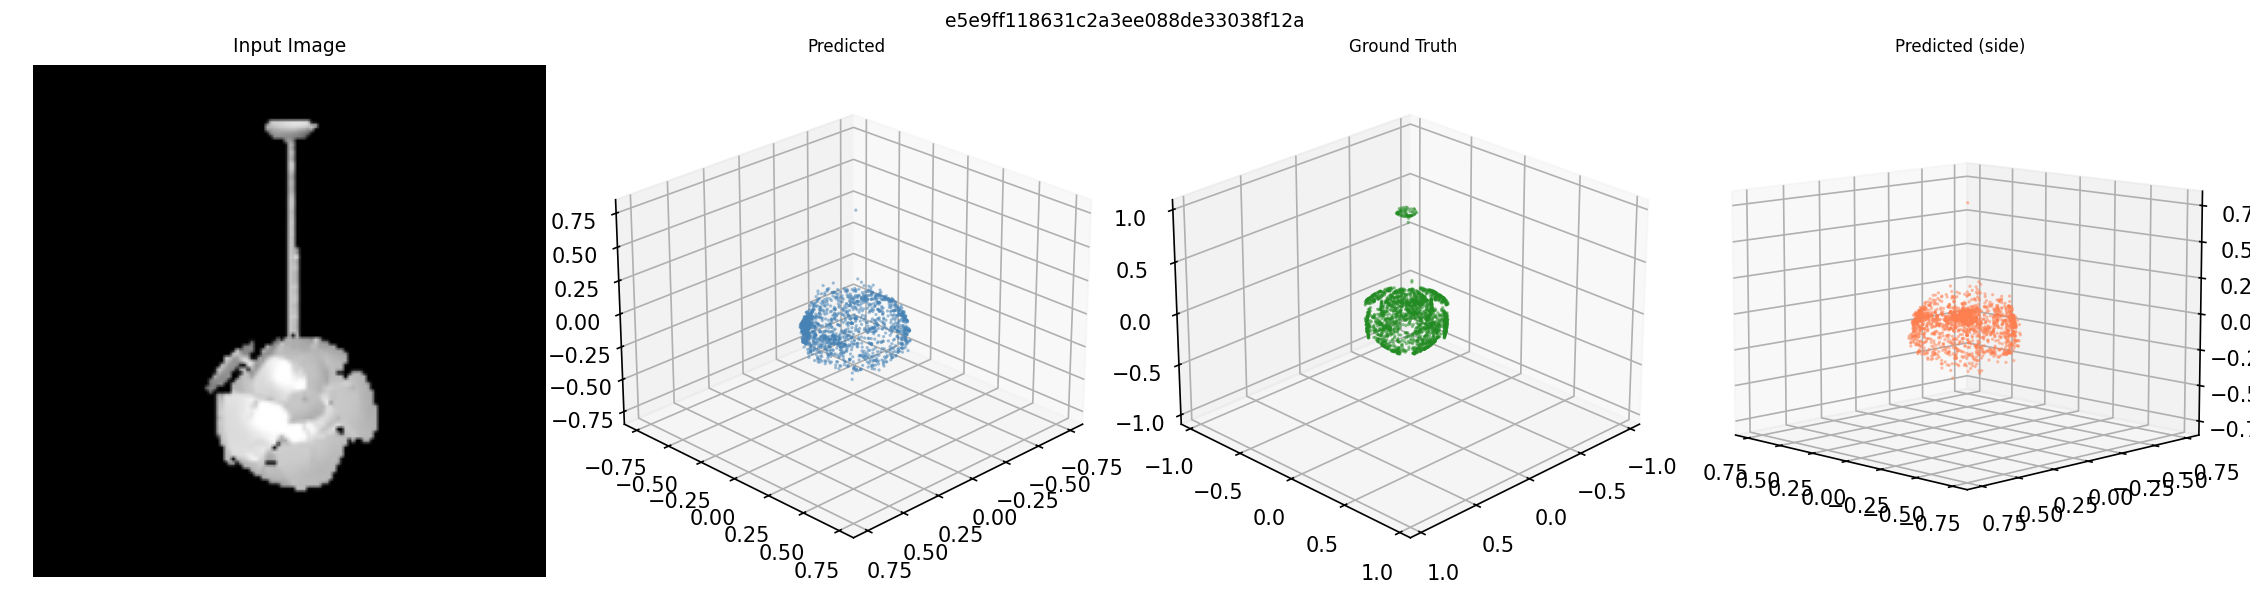
\includegraphics[width=0.24\textwidth]{figures/synth_lamp.png}
\hfill
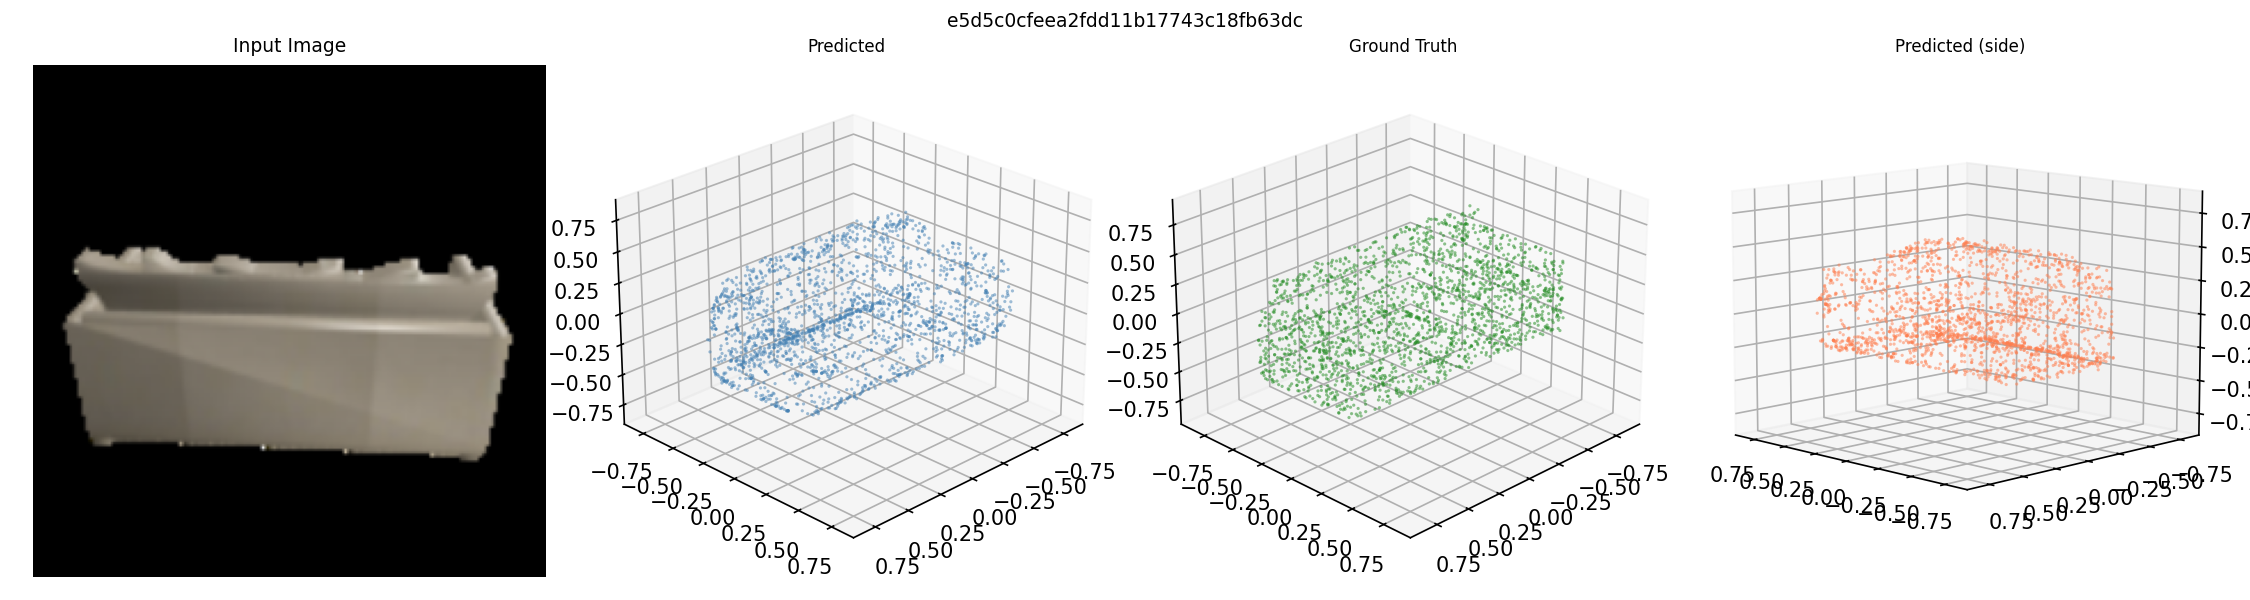
\includegraphics[width=0.24\textwidth]{figures/synth_cabinet.png}
\caption{Synthetic test results. Each panel: input image, predicted point cloud (blue), ground truth (green), and side view. From left to right: airplane, car, lamp, cabinet. The model captures overall shapes accurately.}
\label{fig:synth_results}
\end{figure*}

\begin{figure*}[t]
\centering
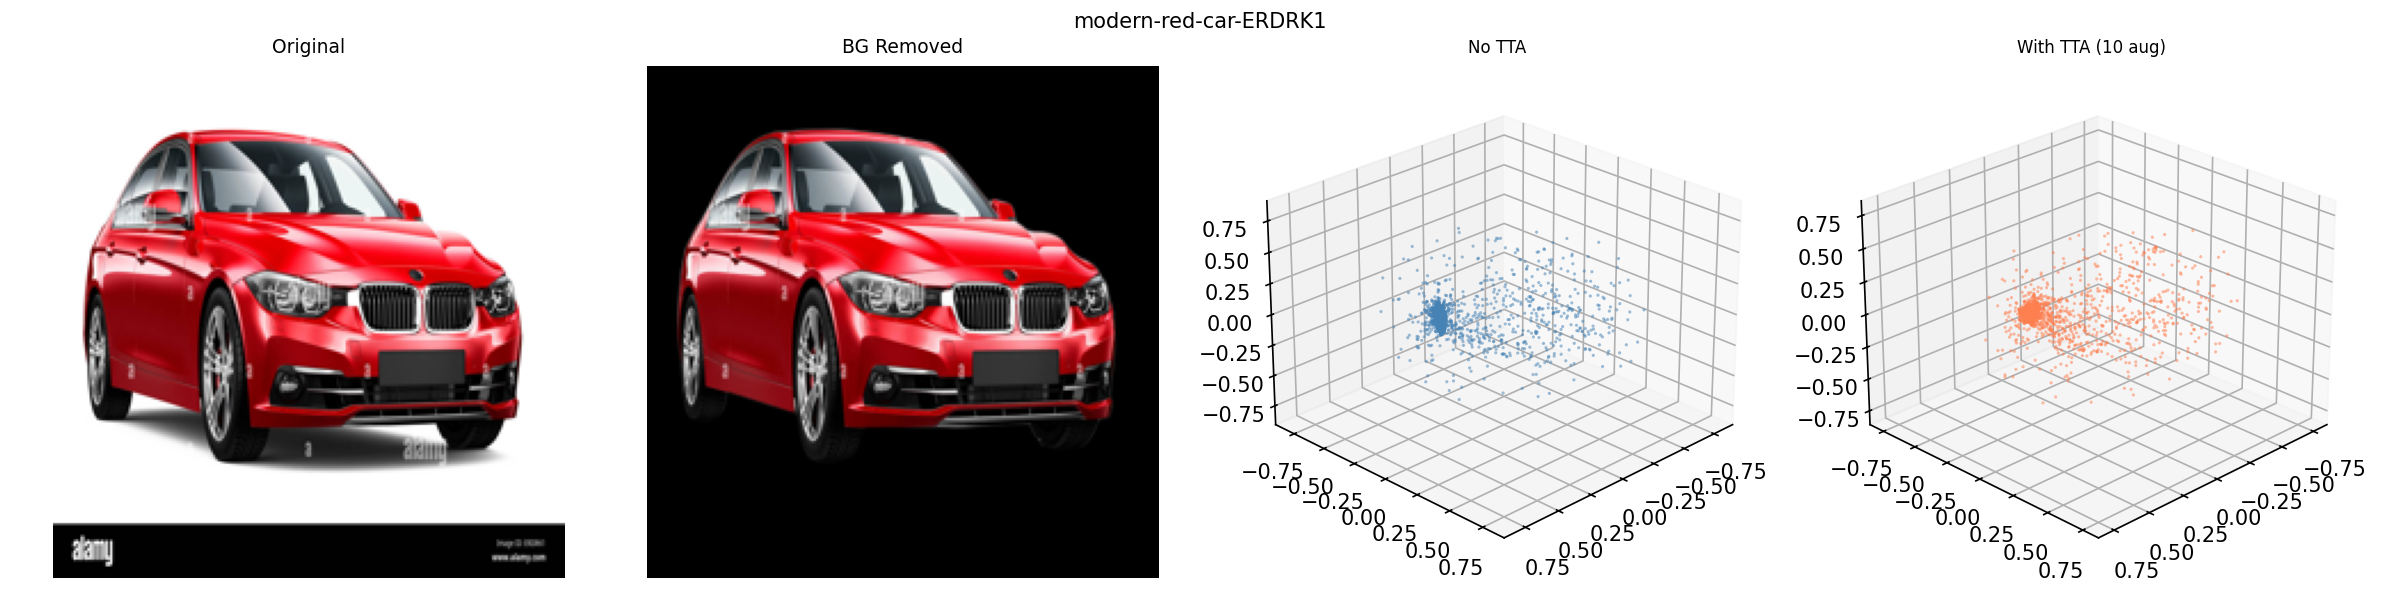
\includegraphics[width=0.24\textwidth]{figures/real_car.png}
\hfill
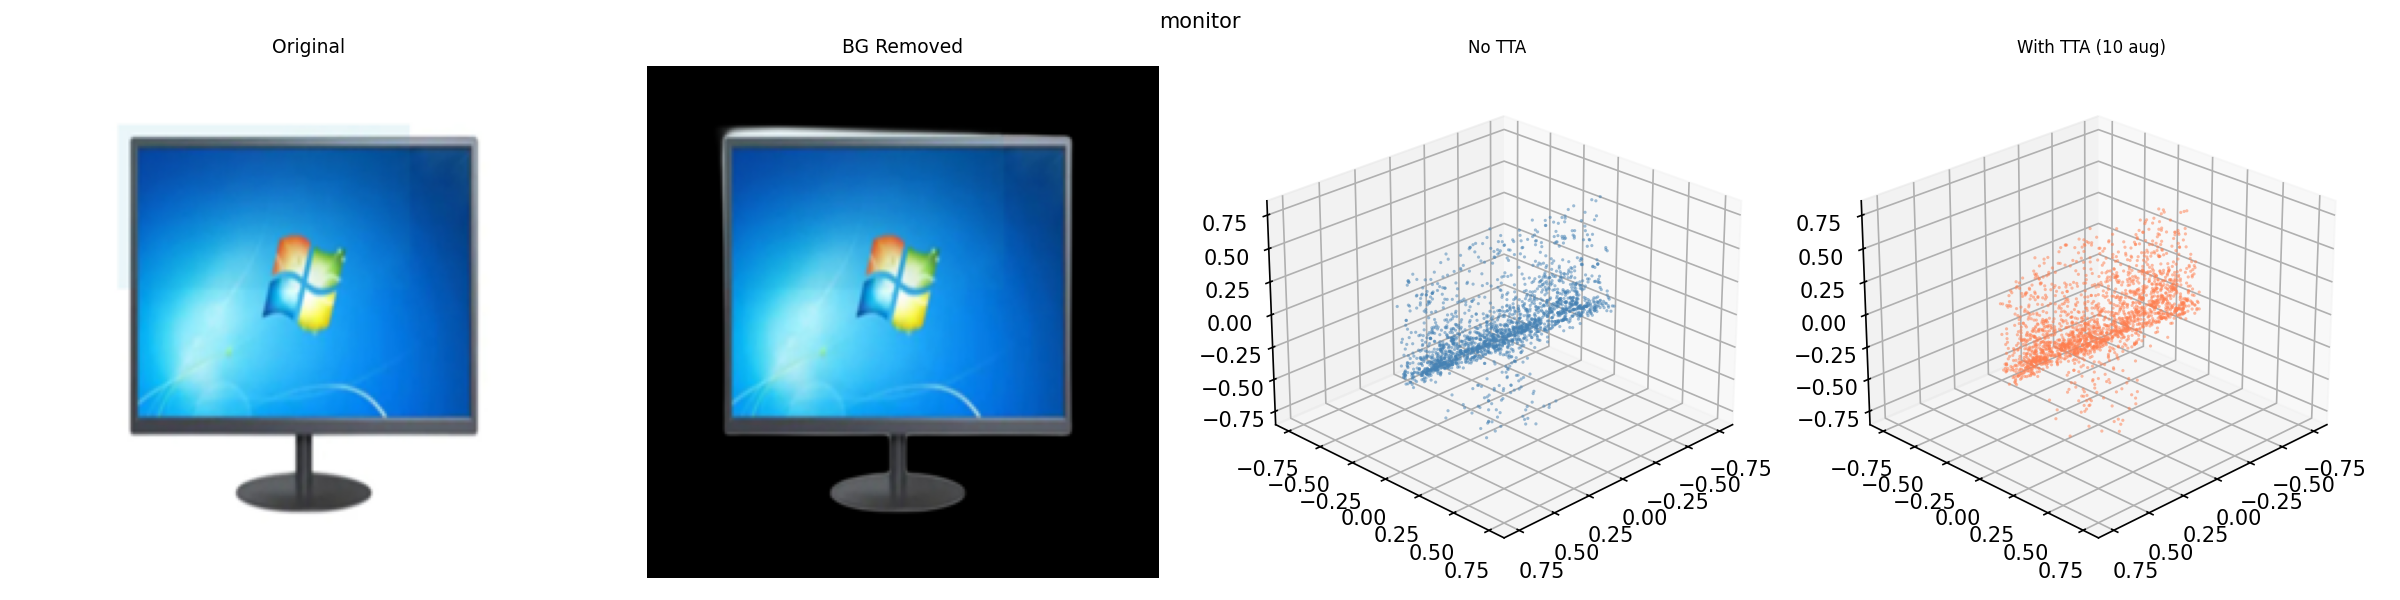
\includegraphics[width=0.24\textwidth]{figures/real_monitor.png}
\hfill
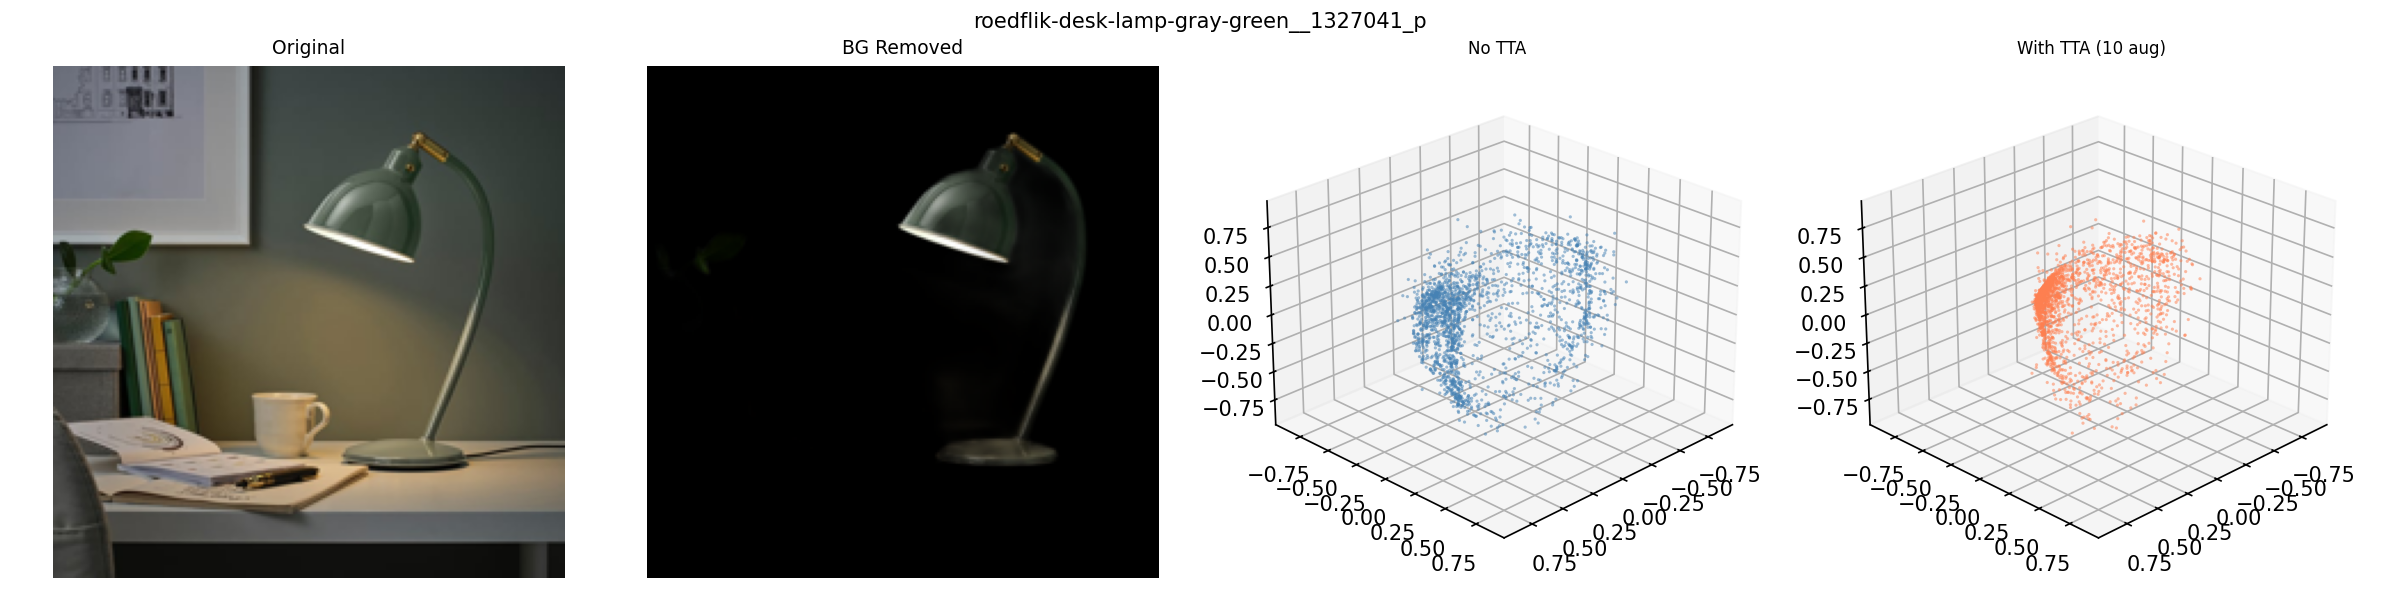
\includegraphics[width=0.24\textwidth]{figures/real_lamp.png}
\hfill
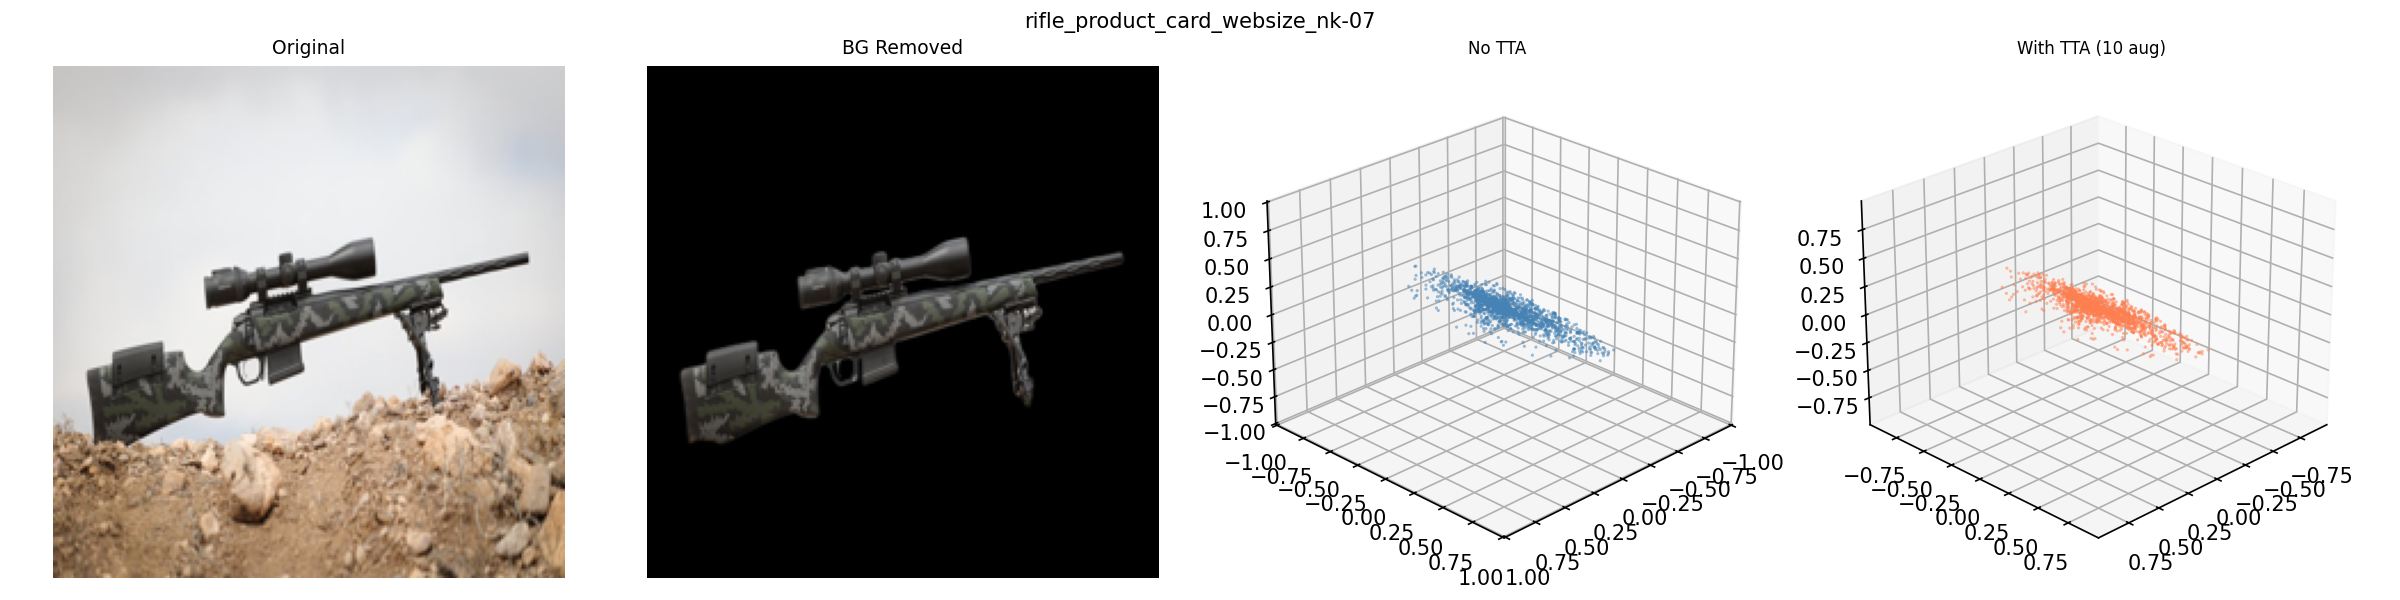
\includegraphics[width=0.24\textwidth]{figures/real_rifle2.png}
\caption{Real-world inference on internet photographs. From left to right: car, monitor, desk lamp, rifle. Background removal + TTA produces recognizable 3D shapes from single images despite never seeing real-world training data.}
\label{fig:real_results}
\end{figure*}

\begin{figure}[t]
\centering
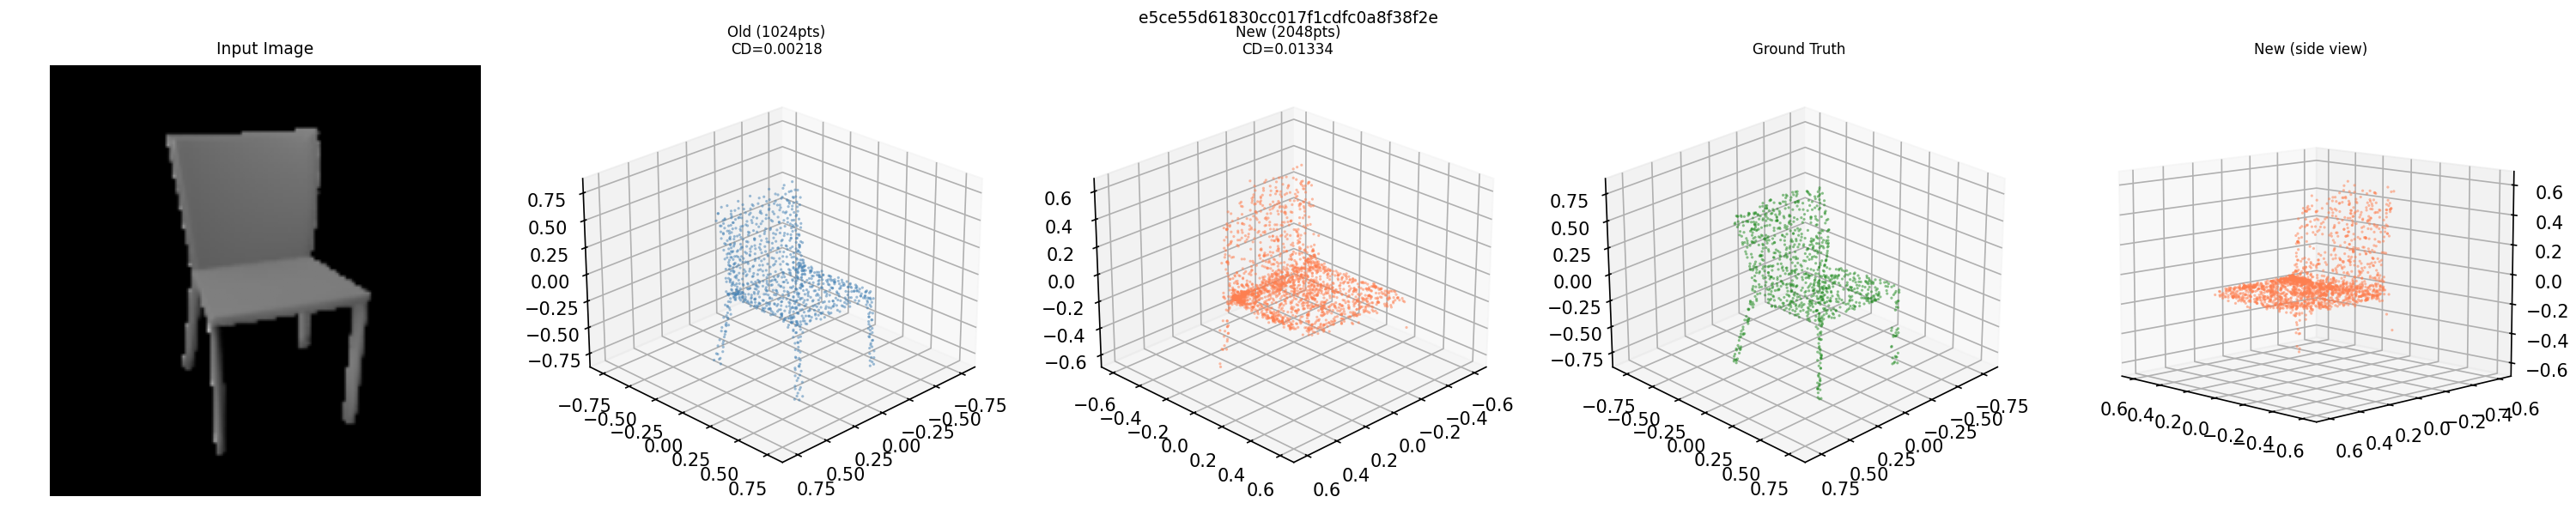
\includegraphics[width=0.48\linewidth]{figures/old_chair1.png}
\hfill
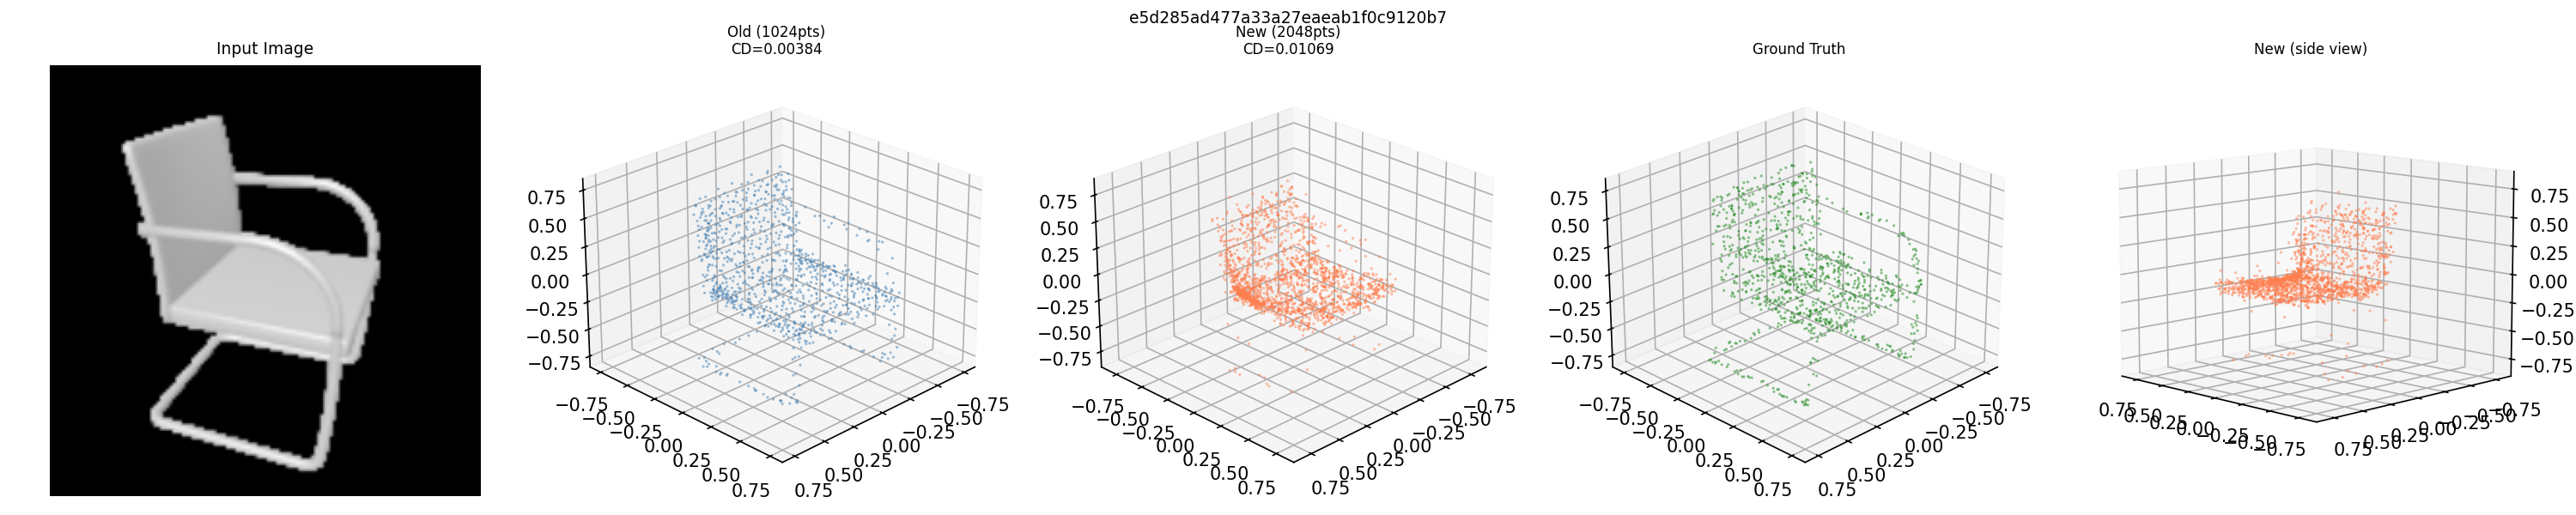
\includegraphics[width=0.48\linewidth]{figures/limitation_chair1.png}
\caption{Chair comparison showing a key limitation. \textbf{Left:} 1024-point model (100 epochs) captures chair legs and structure. \textbf{Right:} 2048-point model (40 epochs) is denser but scattered on thin structures like legs.}
\label{fig:chair_comparison}
\end{figure}

Figure~\ref{fig:chair_comparison} reveals a key limitation: while the 2048-point model achieves better overall metrics, it struggles with thin structures (chair legs, lamp arms) where Chamfer Distance allows spatially spread solutions.

% ===================================================================
\section{Critical Training Bugs}\label{sec:bugs}

During development, we discovered and fixed seven critical bugs that severely impacted model quality.
We document these as practical lessons for the community:

\textbf{1. Flip Augmentation Misalignment.}
\texttt{RandomHorizontalFlip} was applied to input images but \emph{not} to ground truth point clouds.
50\% of training samples had contradictory supervision, causing the model to predict symmetric blobs.
\textit{Fix:} Remove spatial augmentations that cannot be consistently applied to both input and target.

\textbf{2. No Differential Learning Rate.}
Using a single learning rate for both the pretrained encoder and random decoder destroyed ImageNet features in early epochs.
\textit{Fix:} Encoder LR = $0.2\times$ base, decoder LR = $5\times$ base.

\textbf{3. Wrong Loss API Signatures.}
\texttt{chamfer\_distance(pred, gt, reduce='mean')} silently failed --- the correct signature uses \texttt{bidirectional=True}.
Similarly, \texttt{f\_score()} returns a tensor, not a tuple.
This caused validation to crash silently, so the ``best'' checkpoint was actually epoch 0.
\textit{Fix:} Always test loss/metric functions with dummy data before training.

\textbf{4--7.} Additional bugs included: too many self-attention layers (6 $\rightarrow$ 4), warmup/scheduler conflict, constructor parameter error, and a variable name typo.

% ===================================================================
\section{Discussion and Limitations}

\textbf{Pretrained Features Reduce Domain Gap.}
Our key finding is that an ImageNet-pretrained encoder inherently bridges much of the synthetic-to-real gap.
The encoder has already learned to extract features from real-world images, so fine-tuning on synthetic data preserves much of this capability when using differential learning rates.

\textbf{Limitations.}
(1) Chamfer Distance allows spatially spread solutions, struggling with thin structures.
(2) Single-view ambiguity means occluded regions are guessed.
(3) No quantitative real-world evaluation (no real-world 3D ground truth available).
(4) The 2048-point model was only trained for 100 epochs --- longer training would likely improve fine structure prediction.

\textbf{Future Work.}
Earth Mover's Distance or surface-aware losses could improve thin structure reconstruction.
Multi-view fusion at test time could resolve single-view ambiguities.
Training on larger datasets with more categories would improve generalization.

% ===================================================================
\section{Conclusion}

We presented a hybrid CNN-Transformer model for single-image 3D point cloud reconstruction, achieving a 6$\times$ improvement over the Pix2Vox baseline on ShapeNet.
Our systematic evaluation of four domain adaptation strategies shows that test-time augmentation provides the best cost-benefit trade-off for bridging the synthetic-to-real gap.
We demonstrated successful generalization to real-world photographs across multiple object categories.
Our detailed documentation of training bugs provides practical guidance for the point cloud reconstruction community.

% ===================================================================

{\small
\bibliographystyle{ieee}
\bibliography{references}
}

\end{document}
